
\begin{table*}[!hbt]
	\begin{center}
		\caption{Release details from each analyzed project}
		\label{tab:evolution_overview}
		\begin{tabular}{l l| c c c c c c c}
			\toprule
			\textbf{Project}  & \textbf{Release} & \textbf{LOC} & \textbf{Commented lines} & \textbf{Directories} & \textbf{Functions} & \textbf{Statements} & \textbf{Complexity} & \textbf{\# Developers}\\ \midrule              
			\multirow{2}*{Coffeescript}& First  0.6.1                   &           4693 &           836 &           3 &       915 &       5916 &       2958\\
			& Last   1.9.0                   &           7723 &           124 &           6 &      1262 &       6687 &       5251\\ \midrule
			\multirow{2}*{Less.js     }& First  v1.0                    &           1269 &           279 &           6 &       179 &        818 &        634\\
			& Last   v2.3.1                  &          18585 &          2085 &          18 &      2605 &      13609 &       9414\\ \midrule
			\multirow{2}*{Npm         }& First  v0.0.7                  &           1979 &           259 &           3 &       238 &       1234 &        780\\
			& Last   v2.7.4                  &          19837 &          1060 &          34 &      2469 &      12004 &       5918\\ \midrule
			\multirow{2}*{Mongoose    }& First  0.0.1                   &            554 &            12 &           6 &       100 &        373 &        217\\
			& Last   4.0.1                   &          41844 &          5710 &          12 &      5749 &      27722 &       9373\\ \midrule
			\multirow{2}*{Underscore  }& First  1.0.3                   &           1127 &           154 &           2 &       376 &       1317 &        738\\
			& Last   1.8.0                   &           3918 &           385 &           2 &       849 &       3719 &       1650\\ \midrule
			\multirow{2}*{Node-mysql  }& First  v0.1.0                  &           2431 &            55 &           4 &       203 &       1876 &        435\\
			& Last   v2.6.0                  &          10701 &           430 &          16 &      1046 &       8044 &       2010\\ \midrule
			\multirow{2}*{Q           }& First  v0.1.0                  &            188 &            95 &           1 &        35 &        113 &         64\\
			& Last   v1.1.2                  &           6670 &          1149 &           6 &      1396 &       4118 &       2182\\ \midrule
			\multirow{2}*{Request     }& First  v1.2.0                  &            312 &            12 &           2 &        24 &        214 &        112\\
			& Last   v2.54.0                 &           7839 &           333 &           5 &       958 &       4086 &       1713\\ \midrule
			\multirow{2}*{Ember.js    }& First  sc-v2.0.beta.1          &          28582 &         10006 &          67 &      3879 &      21402 &       9743\\
			& Last   v1.11.0-beta.5          &          65548 &         14698 &         115 &      9323 &      38894 &      13878\\ \midrule
			\multirow{2}*{Source-map  }& First  0.1.0                   &           1214 &           855 &           5 &       124 &        669 &        271\\
			& Last   0.4.1                   &           4485 &           791 &           7 &       322 &       2362 &        757\\ \midrule
			\multirow{2}*{Bootstrap   }& First  v1.3.0                  &            886 &           105 &           2 &       130 &        510 &        261\\
			& Last   v3.3.2                  &           6834 &           358 &           5 &       980 &       4532 &       2337\\ \midrule
			\multirow{2}*{Mocha       }& First  0.0.1-alpha1            &           1185 &           284 &           6 &       226 &        703 &        309\\
			& Last   2.2.0                   &           9931 &          2229 &          21 &      1750 &       6586 &       3197\\ \midrule
			\multirow{2}*{Brackets    }& First  sprint-1                &           6271 &          1198 &          14 &      1305 &       4234 &       2183\\
			& Last   release-1.2-prerelease1 &         266801 &         63923 &         179 &     27845 &     148274 &      82848\\ \midrule
			\multirow{2}*{Bower       }& First  v0.1.1                  &           1149 &           117 &           9 &       212 &        856 &        423\\
			& Last   v1.4.0                  &          15802 &          1439 &          17 &      2454 &       8641 &       3646\\ \midrule
			\multirow{2}*{Grunt       }& First  v0.4.0                  &           3972 &           682 &          11 &       492 &       2482 &        886\\
			& Last   v0.4.4                  &           4010 &           663 &          12 &       498 &       2447 &        874\\ \bottomrule
		\end{tabular}
	\end{center}
\end{table*}

\par
We use different metrics listed in Table \ref{tab:metrics_definition} metrics. Table \ref{tab:evolution_overview} shows the difference each project has in terms of metrics in comparison of first and last release.
As we can see Brackets first release contains 6271 lines of code but it ends up with 266801 lines of code in the last release. Bracket's last release is the most biggest evolved project with in four years of its existence. It started with 14 directories which in the last release it contains 179 directories. Brackets has 60 releases during its lifetime with 15871 commits. On the other hand NPM with 298 releases is the project with most releases in our dataset. It starts with 1979 lines of code where the last release exceeds to 19837 lines of code with 2231 functions added since the first release. 

\subsection{Release density}

To better understand the detail of evolution we depict the growth of LOC, directories, functions, statements and complexity. Figure \ref{fig:release_density} exhibit an evolution of our projects.  
\par
Mongoose has fluctuated during its lifetime to the point that it has 24 releases at 2012 while it shows relatively 4 releases in 2014. We can infer that at beginning of its development due to the nature of changes and developer usage they release many versions. After Mongoose became more stable it has less releases per each three month. Bootstrap is one the libraries that has steady increase and decrease in its evolution while it has less release rate in compare to Mongoose. We use following formula to calculate release density in period of three months:
\begin{center}
	$Release Density= \frac{\sum Releases}{3 Months}$
\end{center}

% release_density 
\begin{figure}[thb!]
	\caption{Release density evolution}
	\label{fig:release_density}
	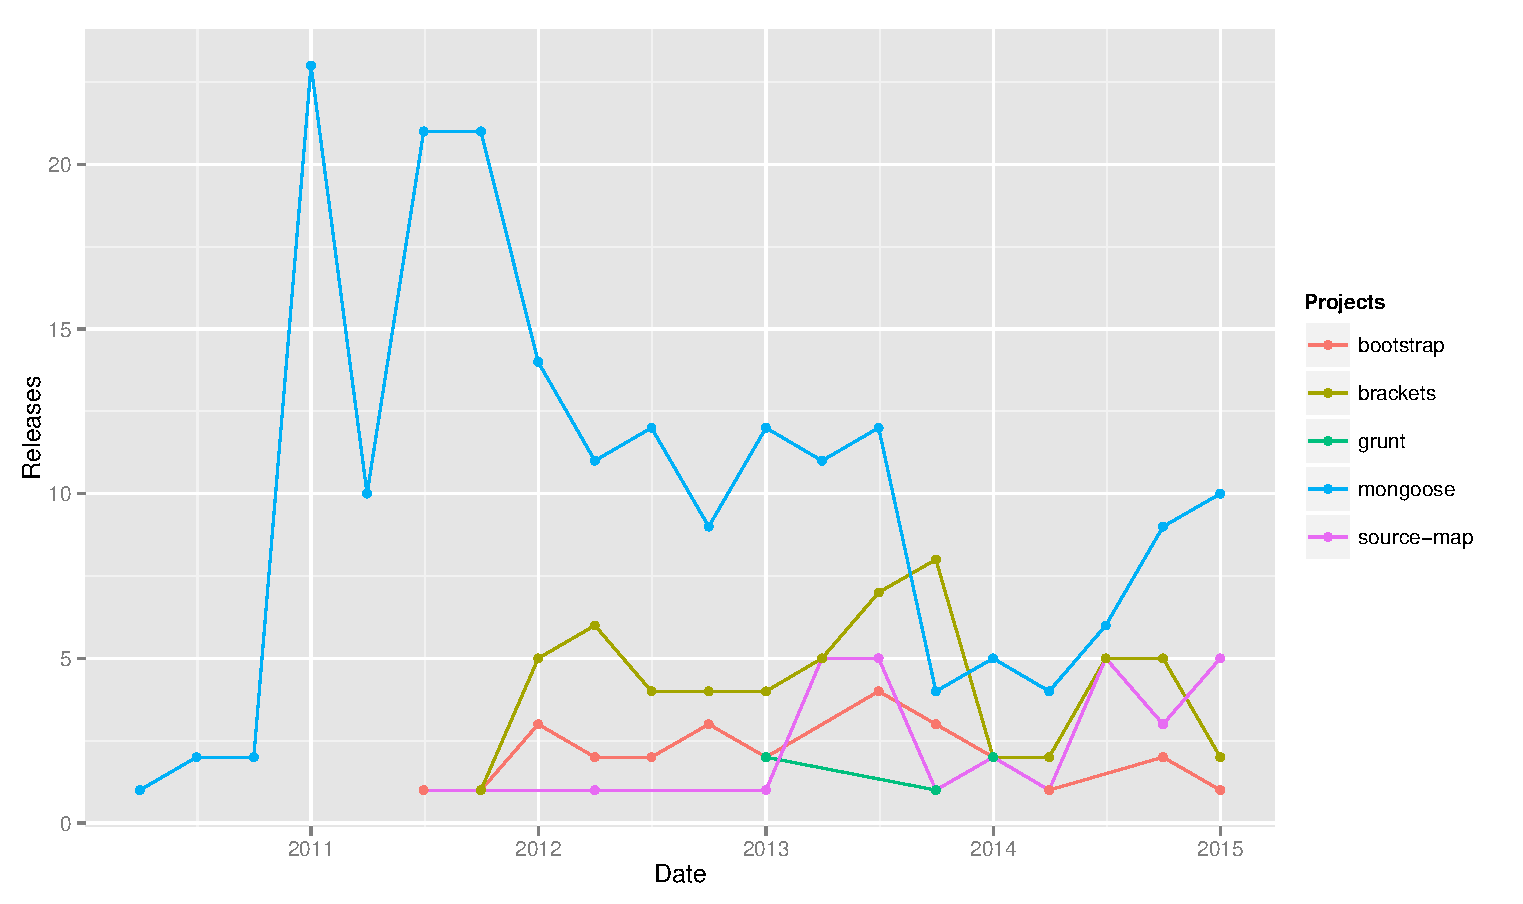
\includegraphics[width=90mm,scale=0.5]{figures/release_density}
\end{figure}





% release_density 
 \begin{figure}[thb!]
 	\caption{Function density evolution}
 	\label{fig:function_density}
 	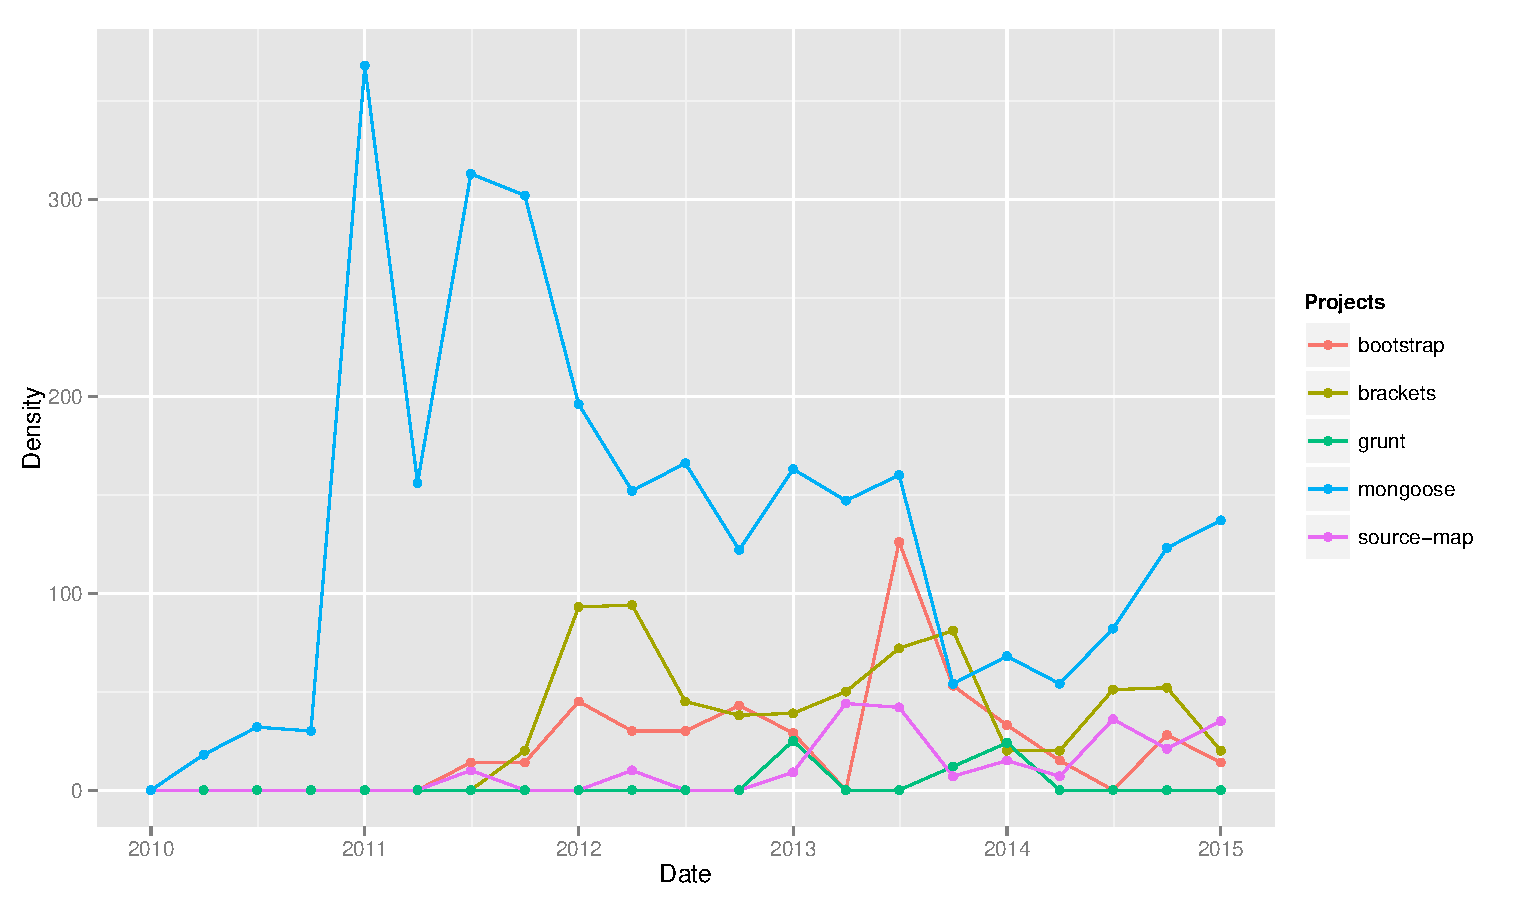
\includegraphics[width=90mm,scale=0.5]{figures/function_density}
 \end{figure}


\subsection{Function density}
We depict the function density of the five chosen projects. We calculated the function density during time periods of three months.
Figure \ref{fig:function_density} indicates evolution of our five selected projects. Mongoose starts at 2010 with almost 17\% function density and it has decreasing trend during its lifetime. It can indicates that after a while developers decided to refactor code to have remove excessive use of functions. Before mid 2012 till 2015 it shows interesting phenomena. The function density keeps same and due to the nature of Mongoose project which is a object modeling for MongoDB there were no any changes in their APIs. Generally APIs exposed by function declarations and function expressions in JavaScript. So the API keeps unchanged for a long period. We calculate function density as following:

\begin{center}
	$Function Density=  \frac{\left ( \frac{Number Of Functions}{Lines Of Code} \right)}{Number Of Releases}\ast 100$
\end{center}

\par
Like Mongoose we have the same trend for Brackets which after a sharp decline during 2012 to 2013 the function density becomes unchanged for two years. These trends, again revealed projects become mature and established that they do not need to change their API. One might argue these project would be stop developing and the behavior is because they are in maintenance phase. But We have numerous release in each period and we cannot say these projects are abandoned.  
 


\par For number of developers we tried to gather data based on email of authors that commit code, however we found out that authors can have multiple emails register to one login id. As a result we tried to count the number of developers based on the Github usernames. 


\par
Having comments as one of the artifacts that can improve the readability of source code we examined it as metric of evolution.
Brackets has the most comment lines with having 63923 comment lines followed by Ember.js with 14698 comment lines. The least documented project is CoffeeScript with having only 124 lines of documentation. What makes the resuls interesting, is the fact that CoffeeScript starts with 836 lines of comments in the first release but in the last release we have only 124 lines of code. CoffeeScript and Grunt are the only projects that adapt this pattern, while all the other projects show growing trend in number of comments during evolution.  


\subsection{Number of developers in each release}
The next characteristics we measure in evolution is to measure how much a project is community driver. We count number of developers having at least one commit in each period between releases. Figure \ref{fig:number_of_developers} and and . Request and Bootstrap are among projects with over 80 and 100 developers at individual peaks in development phase. Despite the fact that Underscore has fluctuated while evolving, at recent releases it shows that it gains some more attention and it becomes more community driven. Project q takes less attention as compare to other projects. It has never had more than 20 developers since its beginning in mid 2010.
\par
Request project has one drastic fell down in mid 2013. When we explore that we found that they two release really closed to each other. The first one has more than 80 developers while the other has less 10 developers. This indicates that they found some major issues in former issue and few core developers instantly fix them and they released another version. One interesting phenomena that we observe is that number of released skewed to the right of each graph. Best practices in software engineering suggest having iterative and incremental development. Based on this fact we guess developers tend to have more smaller release in time rather than having one huge release every 6 months.  
% release_density 
\begin{figure}[thb!]
	\caption{Number of developers per release}
	\label{fig:number_of_developers}
	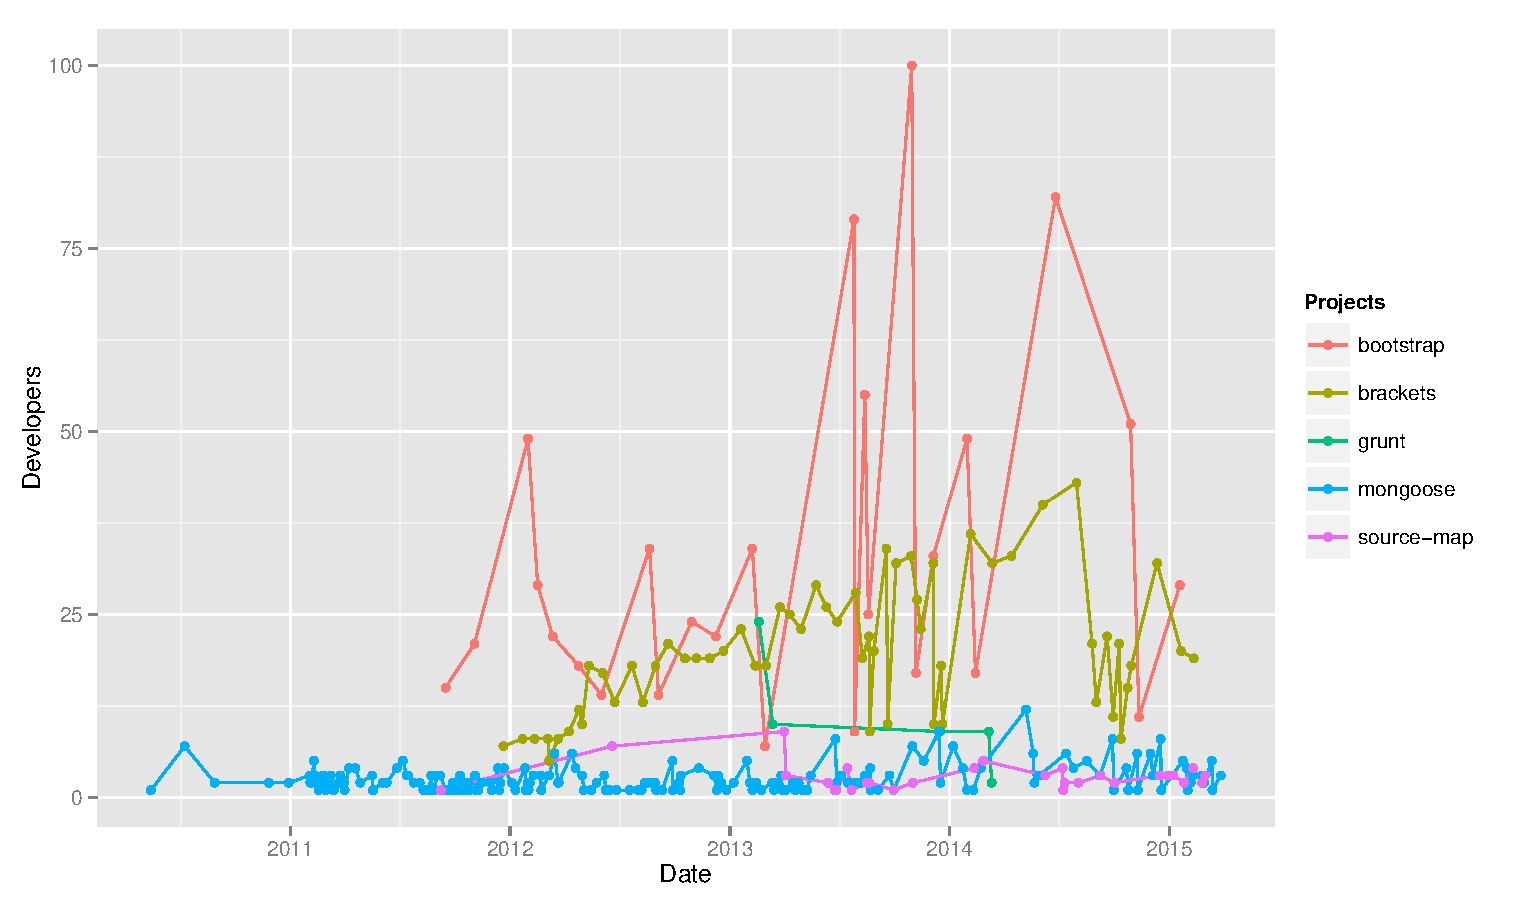
\includegraphics[width=90mm,scale=0.5]{figures/number_of_developers}
	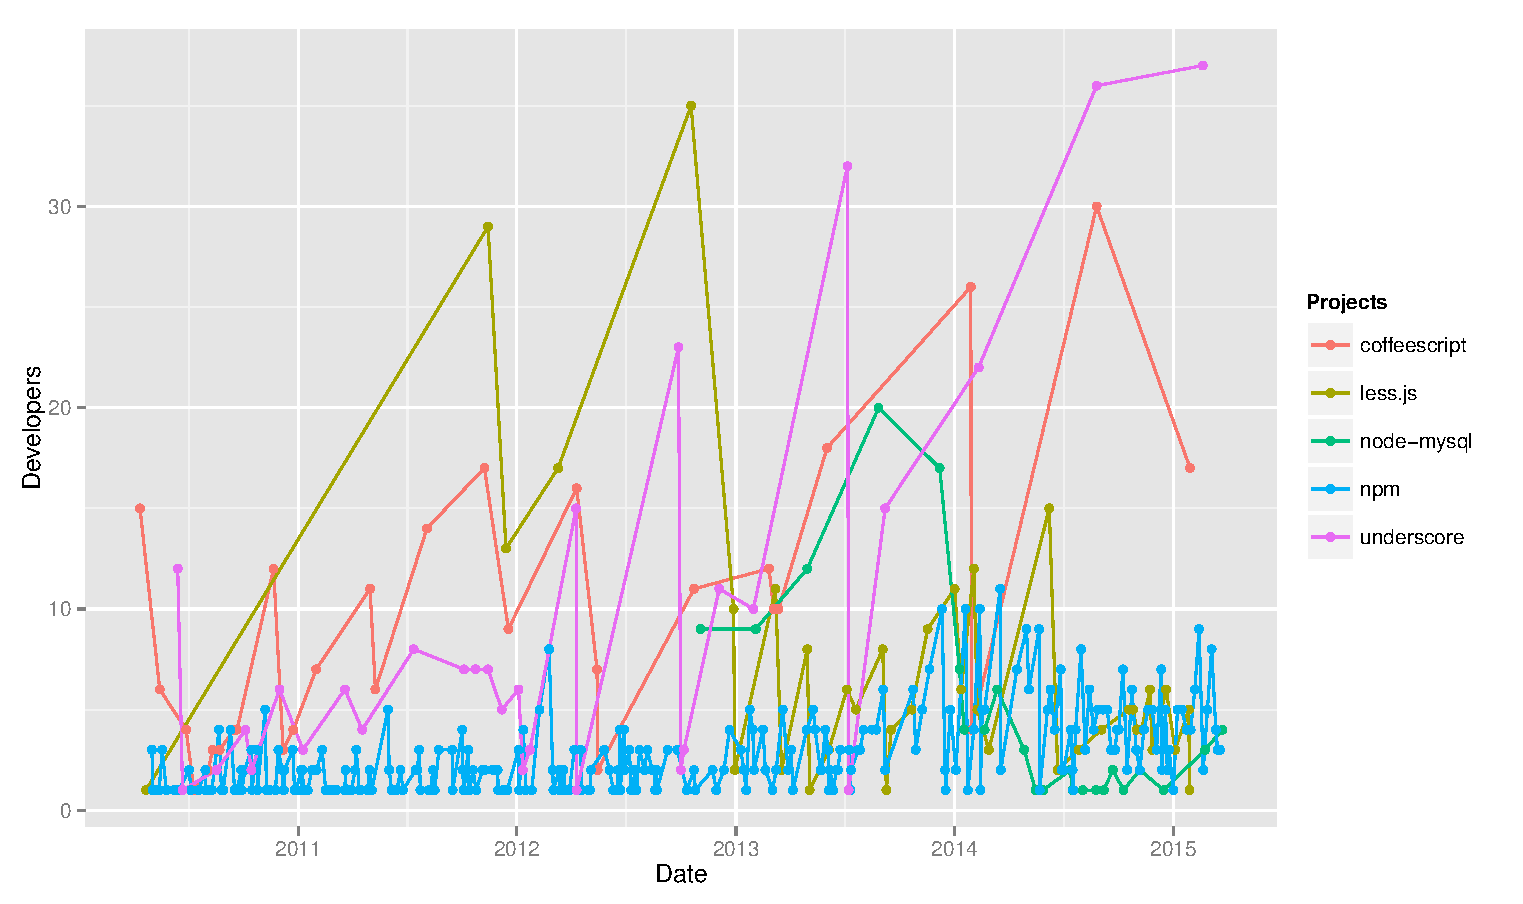
\includegraphics[width=90mm,scale=0.5]{figures/number_of_developers_2}
		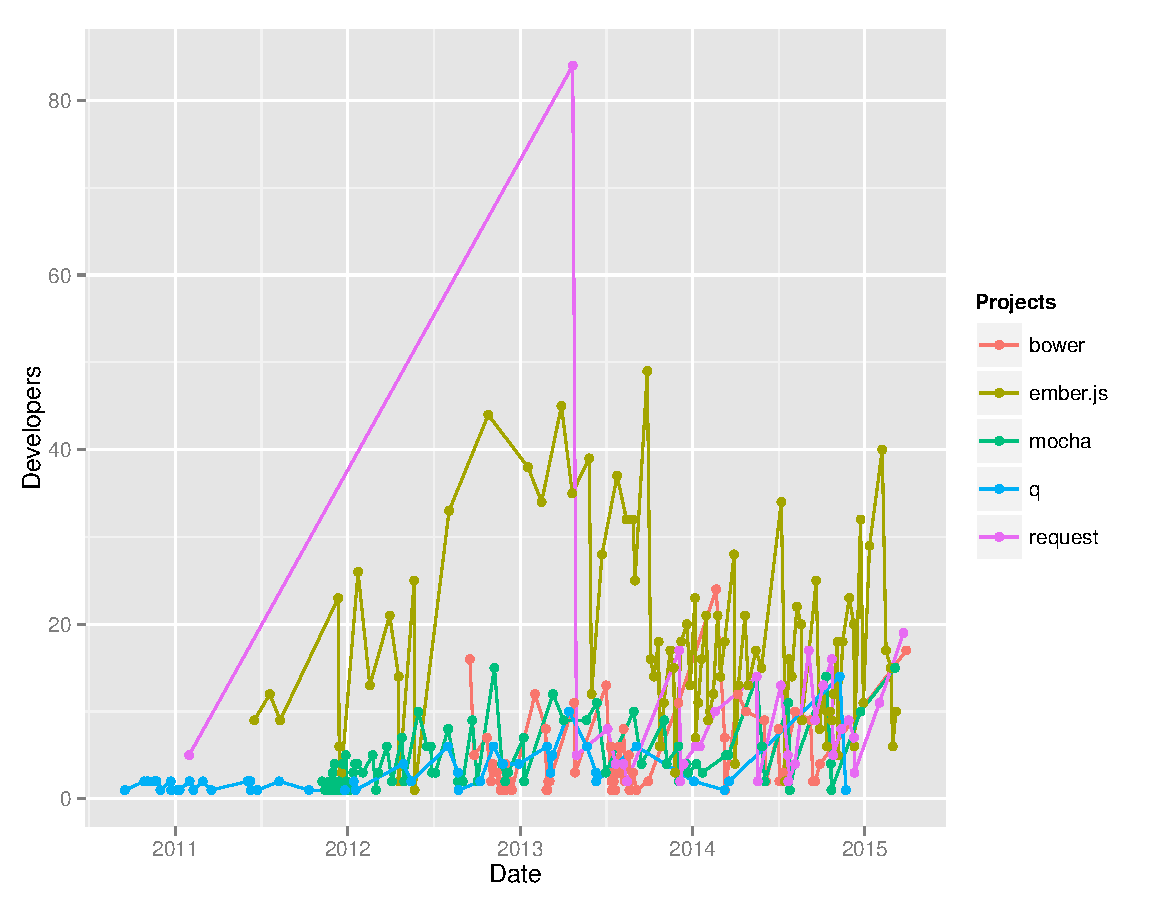
\includegraphics[width=90mm,scale=0.5]{figures/number_of_developers_3}
\end{figure}

\subsection{Issues per release}


\ref{fig:number_of_issues}
Having a software without bug means that software is never used by users. When it comes to bugs, we can find where and in what extent the software's problem are saturated. The module or component with more issues indicate that module is either too complex or is used directly by user and other components. Taking a look in each project and density of issues during releases can get us an insight into the details of projects. Figure \ref{fig:number_of_issues} shows numbers of issues introduced between releases.

\begin{figure}[thb!]
	\caption{Number of issues introduced in each release}
	\label{fig:number_of_issues}
	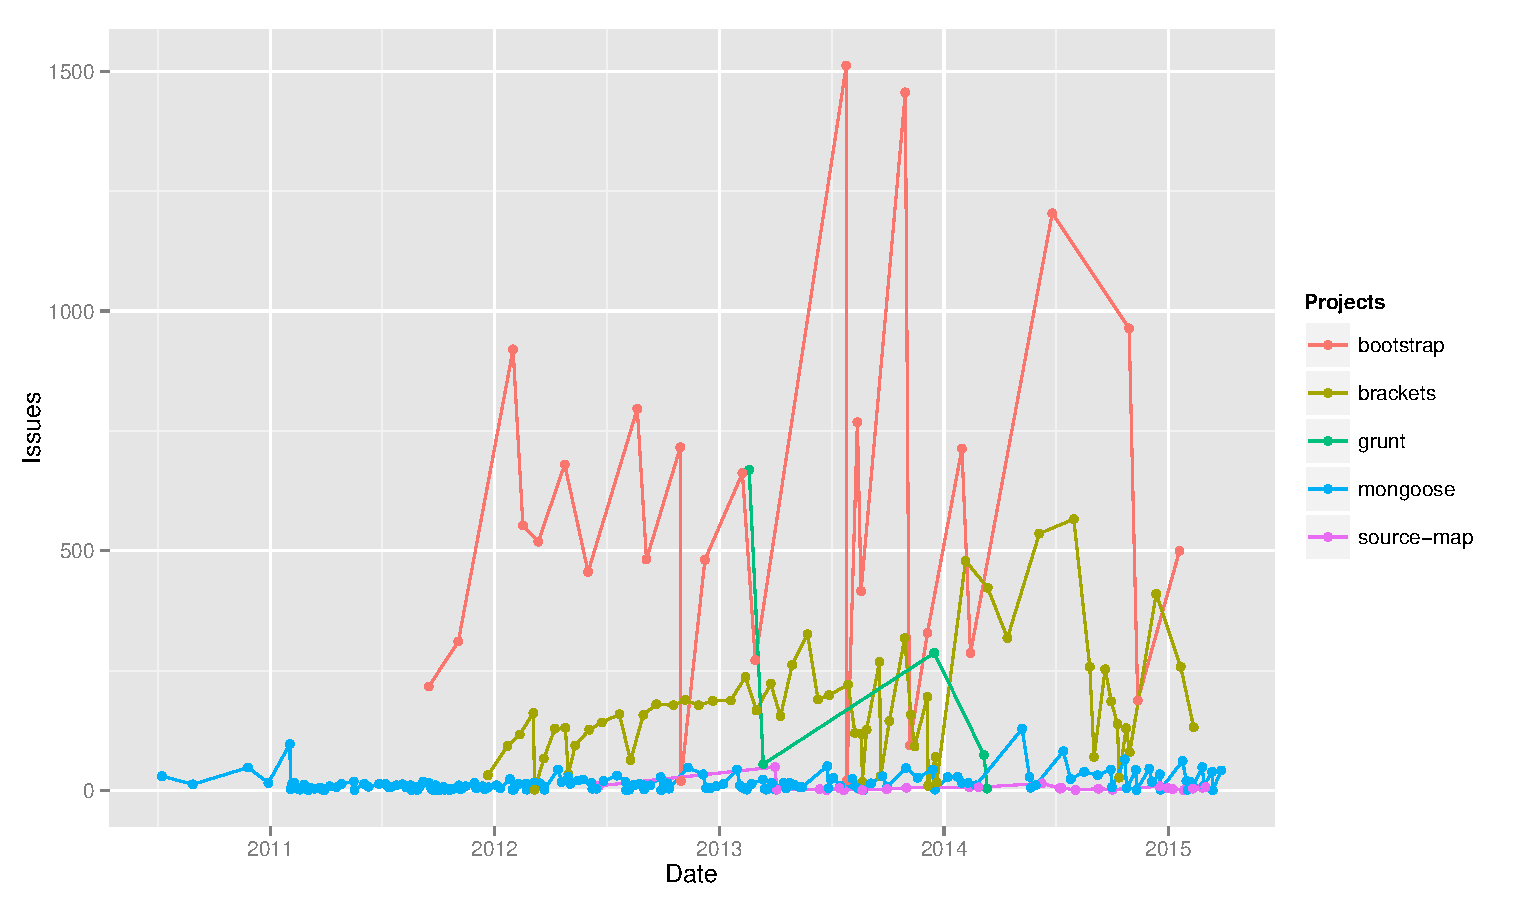
\includegraphics[width=90mm,scale=0.5]{figures/issues_per_release}
	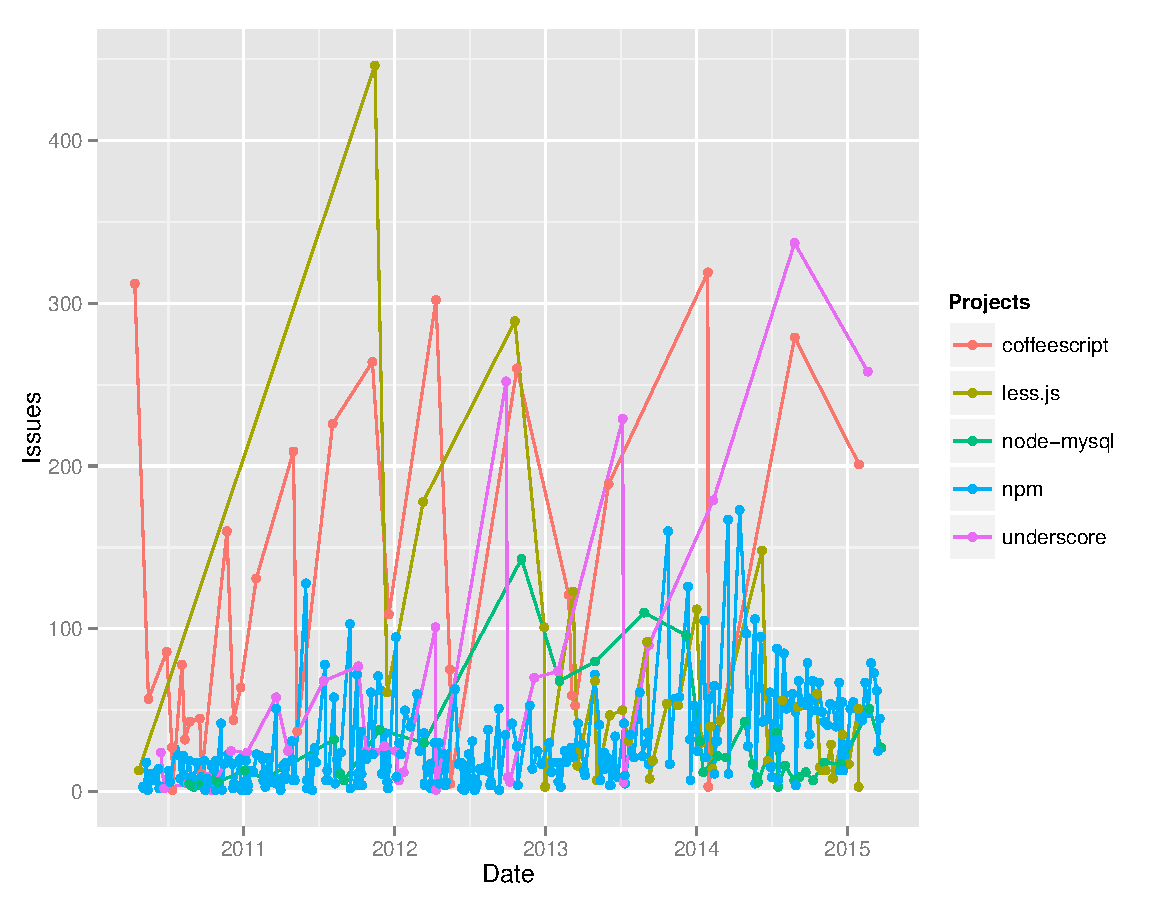
\includegraphics[width=90mm,scale=0.5]{figures/issues_per_release_2}
	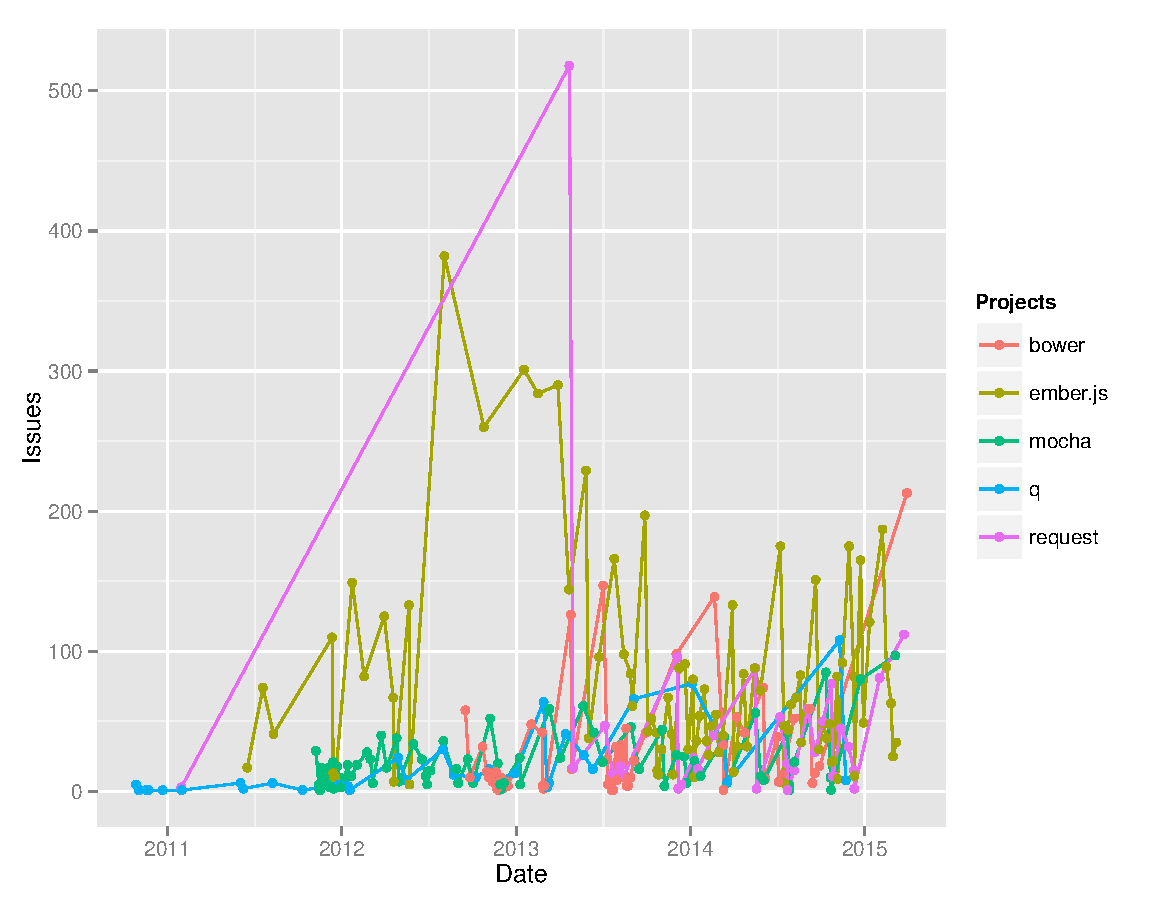
\includegraphics[width=90mm,scale=0.5]{figures/issues_per_release_3}
\end{figure}

By looking at the graph we can infer Bootstrap in special releases had around 1000 issues caught by testers and developers. Looking back to the nature of this project, it is obvious such a huge library which provides lots of functionalities can have numerous users whom they can report bugs while using this library in different scenarios. Moreover for the release in the mid of 2013 we can see the distance between that release and previous ones was significant. By looking at the data we found out that was one of the major releases that Bootstrap had. 

\begin{table}[!hbt]
	\begin{center}
		\caption{Average time to fix a bug}
		\label{tab:average_time_bugfix}
		\begin{tabular}{l| c }
			\toprule
			\textbf{Project}  & \textbf{Average bug fix in days} \\ \midrule              
			Coffeescript    & 46  \\
			Less.js         & 113 \\
			Npm             & 58  \\
			Mongoose        & 44  \\
			Underscore      & 14  \\
			Node-mysql      & 47  \\
			Q               & 30  \\
			Request         & 105 \\
			Ember.js        & 22  \\
			Source-map      & 17  \\
			Bootstrap       & 11  \\
			Mocha           & 83  \\
			Brackets        & 26  \\
			Bower           & 30  \\
			Grunt           & 28  \\  \bottomrule
		\end{tabular}
	\end{center}
\end{table}

To study more about these different projects we conduct another analysis to find the average time it takes to fix a bug that reported after releases. We use Github issue tracker to extract all information related to bugs and we grouped them by releases. Then the average time it takes since the bug was created to the date it closed is calculated. Table \ref{tab:average_time_bugfix} shows the result that the average time in days that it takes to fix bugs in each of selected projects.  
\par 
What we found is that Bootstrap has the least number of days taken to fix a bug. Combining number of developers Bootstrap has based on Figure \ref{fig:number_of_developers} we found that this project has one of the most active communities among other projects. Less.js is a project that on average it takes 113 days to get a bug fixed. 
\par
Underscore has also a good response and fixed rate among projects. While we are comparing the rate of fixing a bug, we observe that Underscore is also one of the projects that has large number of developers contributing to the project. Having deeper observation into the data, we found out that number of developers are correlated to the time it takes to fix and close a bug.

\par For project \textit{q} it takes on average 30 days to fix bugs. By looking at number of developers we found out it has comparably less developers as compare to other projects but we have to take into account scale of project vary. A project that has few functionality migh has fewer bugs and as a consequence fewer time would it take to fix a bug. 

\subsection{JavaScript Rule violations}
Using SonarQube various rules for finding code smells in JavaScript projects we are able to extract code smells with different severity. To explain it more we list following rules:

\begin{itemize}
	\item \textbf{"===" and "!=="}:
The == and != operators do type coercion before comparing values. This is bad because it can mask type errors. For example, it evaluates \escape{t} \escape{r} \escape{n} == 0 as true.

It is best to always use the side-effect-less === and !== operators instead. This issue is considered as \textit{Major} issue.

		\begin{lstlisting}[caption=Noncompliant Code Example]
		if (var == 'howdy') {...} // Noncompliant
		\end{lstlisting}
		
		\begin{lstlisting}[caption=Compliant Solution]
		if (var === 'howdy') {...}
		\end{lstlisting}


	\item \textbf{\textit{continue} should not be used}
	continue is an unstructured control flow statement. It makes code less testable, less readable and less maintainable. Structured control flow statements such as if should be used instead. We considered this issue as \textit{Critical} issue.
	
		
		\begin{lstlisting}[caption=Noncompliant Code Example]
		for (i = 0; i < 10; i++) {
		if (i == 5) {
		continue;  /* Non-Compliant */
		}
		alert("i = " + i);
		}
		\end{lstlisting}
		
		\begin{lstlisting}[caption=Compliant Solution]
		for (i = 0; i < 10; i++) {
		if (i != 5) {  /* Compliant */
		alert("i = " + i);
		}
		}
		\end{lstlisting}
	
	
	
	
	\item \textbf{ \textit{switch} statements should end with a \textit{default} clause}
	he requirement for a final default clause is defensive programming. The clause should either take appropriate action or contain a suitable comment as to why no action is taken. It is a \textit{Major} issue.
	

		
		\begin{lstlisting}[caption=Noncompliant Code Example]
		switch (param) {  //missing default clause
		case 0:
		 doSomething();
		break;
		case 1:
		 doSomethingElse();
		 break;
		}
		
		switch (param) {
		 default: // default clause should be the last one
		 error();
		 break;
		case 0:
		 doSomething();
		 break;
		case 1:
		 doSomethingElse();
		 break;
		}
		\end{lstlisting}
		
		\begin{lstlisting}[caption=Compliant Solution]
		switch (param) {
		case 0:
		 doSomething();
		 break;
		case 1:
		 doSomethingElse();
		 break;
		default:
		 error();
		 break;
		}
		\end{lstlisting}	
	
	
	\item \textbf{\textit{with} statements should not be used}
	The use of the with keyword produces an error in JavaScript strict mode code. However, that is not the worst that can be said against with.
	
	Using with allows a short-hand access to an object's properties - assuming they are already set. But use with to access some property not already set in the object, and suddenly you are catapulted out of the object scope and into the global scope, creating or overwriting variables there. Since the effects of with are entirely dependent on the object passed to it, with can be dangerously unpredictable, and should never be used. It is a major issue.
	
		\begin{lstlisting}[caption=Noncompliant Code Example]
	var x = 'a';
	
	var foo = {
		y: 1
	}
	
	with (foo) {  // Noncompliant
		y = 4;  // updates foo.x
		x = 3;  // does NOT add a foo.x property; updates x var in outer scope
	}
	print(foo.x + " " + x); // shows: undefined 3
		\end{lstlisting}
		
			\begin{lstlisting}[caption=Compliant Solution]
			var x = 'a';
			
			var foo = {
			 y: 1
			}
			foo.y = 4;
			foo.x = 3;
			
			print(foo.x + " " + x); // shows: 3 a
			\end{lstlisting}
			
		
	\item \textbf{Statements should be on separate lines}
	For better readability, do not put more than one statement on a single line. It is a minor issue.
	
	\begin{lstlisting}[caption=Noncompliant Code Example]
	if(someCondition) doSomething();
	\end{lstlisting}
	
	\begin{lstlisting}[caption=Compliant Solution]
if(someCondition) {
doSomething();
}
	\end{lstlisting}
	
	
\end{itemize}
